\documentclass[12pt,a4paper,twoside,openright,bibliography=totocnumbered]{report}

\usepackage{ragged2e}
\usepackage{tikz, pgfplots}
\usepackage{graphicx}
\usepackage{multicol}
\usetikzlibrary{positioning,shapes}
\usepackage{graphicx}
\graphicspath{{./reportImages/}}
\usepackage{geometry}
\usepackage{listings}
\usepackage{amsmath}
\usepackage{tcolorbox}
\usepackage{enumitem}
\usetikzlibrary{arrows.meta, positioning}
\usepackage{amssymb}
\usepackage{setspace}
\usepackage{titlesec}
\usepackage{times}
\usepackage{tocbibind}
%\usepackage[usenames,dvipsnames]{xcolor} % to access some named colors used with \highLight
%\usepackage{luacolor} % required to use the lua-ul \highLight command
%\usepackage{lua-ul}

%\LuaULSetHighLightColor{Aquamarine}

\geometry{margin=1in}

\lstdefinestyle{st1}{
	numbers=left,
	tabsize=2
}

\lstset{style=st1}

\title{Optimizing Computational Graphs Using Relaxed Graph Substitutions}

\author{Kaushik Bhowmick\\ \texttt{u21cs022@coed.svnit.ac.in}
		\and
		Himanshu Thakur\\ \texttt{u21cs046@coed.svnit.ac.in}
		\and
		Bhavya Hirani\\ \texttt{u21cs100@coed.svnit.ac.in}
		}

\date{\today}

\onehalfspacing

\begin{document}
%\maketitle

%\begin{center}
%{ \Large \bfseries Building a test case for Interprocedural GVN } \\
%\end{center}

\begin{singlespace}
\begin{footnotesize}
\begin{abstract}
	\textit{Most deep learning compilers use a greedy approach to optimizing computational graphs in that every successive graph substituion must result in a strict performance increase. This narrows the space of possible optimizations and motivates the notion of relaxed graph substitutions: substitutions that don't themselves result in a more optimal graph version, but facilitate further transformations down the line that ultimately yield a net improvement in performance. In order to determine the pipeline of transformations to be applied such that the net performance increase is guaranteed, we search the space of potential optimizations using a backtracking algorithm which, at a given iteration, determines the cost of the corresponding intermediate graph using programmer-defined heuristics. To test our optimaztion strategy, we plan to implement our own graph transformations in ONNX and we limit our performance heuristics to simply measuring execution time. So far we have created arbitrary computation graphs in ONNX and furthermore successfully implemented the 'enlarge kernel size' transform on it. We have unpacked the theoretical the details of two more transforms - fusing two convolutional layers and fusing an add and convolutional layer. Implementing these will be our next move. Furthermore, we have implemented a cost based backtracking algorithm, but its integration with ONNX computation graph is a further step in implementation.}\\
\end{abstract}
\end{footnotesize}
\end{singlespace}

\tableofcontents

\listoffigures

\titleformat{\chapter}[display]
        {\normalfont\Large\bfseries\centering}
        {\chaptertitlename\ \thechapter}
        {20pt}{\Large}

\titleformat{\section}[hang]
        {\normalfont\normalsize\bfseries}{\thesection}{0.5em}{}

\titleformat{\subsection}[hang]
        {\normalfont\small\bfseries}{\thesubsection}{0.5em}{}


\chapter{Introduction}
%{\large \noindent \bfseries  Introduction}\\
In most Deep Learning frameworks, training and inference are both represented using \textit{Computation Graphs}, where nodes represent operations, and edges represent the flow of data through those operations. Particularly, we can think of each incoming edge for some node N representing arguments to N, each argument being the result of computing the respective subgraphs they are the roots of. Computation graphs, like other programs, can usually be optimized for some metric such as optimal memory usage or efficiency, and has motivated a vast body of literature surrounding the same. That being said, most, if not all, optimizations being worked on so far have been \textit{greedy} in nature. i.e. They optimize a program in \textit{passes}, where each pass, i, goes over the program in order to make some transformation $T_i$, such that $T_i$ \textit{must} lead to a strict performance increase. 

The described constraint restricts the space of transformations an algorithm must explore, and, presumably, sacrifices a hard-to-discern, but ``globally optimal'' solution for a possibly locally optimal option that is guaranteed to improve performance within some time constraint. The idea behind \cite{jia2019} is that it's very feasible to search in a much bigger search space of what are called \textit{relaxed graph substitutions}, leading to a discovery of complex substitutions that go through potentially sub-optimal intermediate steps (hence, ``greedy'') to reach an ultimate resultant computation graph that is better than what we would have achieved using greedy strategies.

The approach presented here is a backtracking algorithm that searches the exhaustive space of intermediate graphs obtained by applying all possible transformations on them (regardless of reducing performance, assuming the reduction in performance is below a set tolerance criteria). To quantify the performance of these intermediate graphs, so as to compare it with its predecessor, successor and other interemdiate transformations, we also need a \textit{cost model} that allows us to statically estimate the same.

\section{Objectives}
Our objectives with this project are two fold:
\begin{enumerate}
	\item Replicate results obtained by \cite{jia2019}, but without the graph splitting algorithm (used to scale the aforementioned non-greedy approach for large graphs)
	\item Flesh out the \textit{cost model} which statically estimates performance metrics on intermediate graphs.
\end{enumerate}
	
\noindent The report is organized as follows:
Chapter 2 gives some theoretical background on deep learning compilers and our motivation for exploring this particular thread of research. Chapter 3 gives some detail about our algorithm, including an in-depth explanation on a running example that we plan to impement as a demonstration of the algorithm. Chapter 4 provides some insight into possible challenges one can face when implementing such a scheme, along with future directions we plan to follow. Chapter 5 summarizes and concludes our exposition.


%We use an example from a ResNet \cite{he2016} module ( figure \ref{resnet} ) to illustrate our strategy. Each arrow represents a graph substitution that produces a graph \textit{equivalent} to its input, where equivalence is defined as the following: two graphs $\mathcal{G}_1$ and $\mathcal{G}_2$ are said to be equivalent if they produce the same outputs for an arbitary input. The first substitution pads a 1x1 convolutional kernel to form a 3x3 one, potentially reducing the performance by introducing more operations. However, doing so enables further node fusions which, as we can see, results in a computational graph giving better performance than what we started with. \\


%\begin{figure}[b!]
	%\begin{center}
		%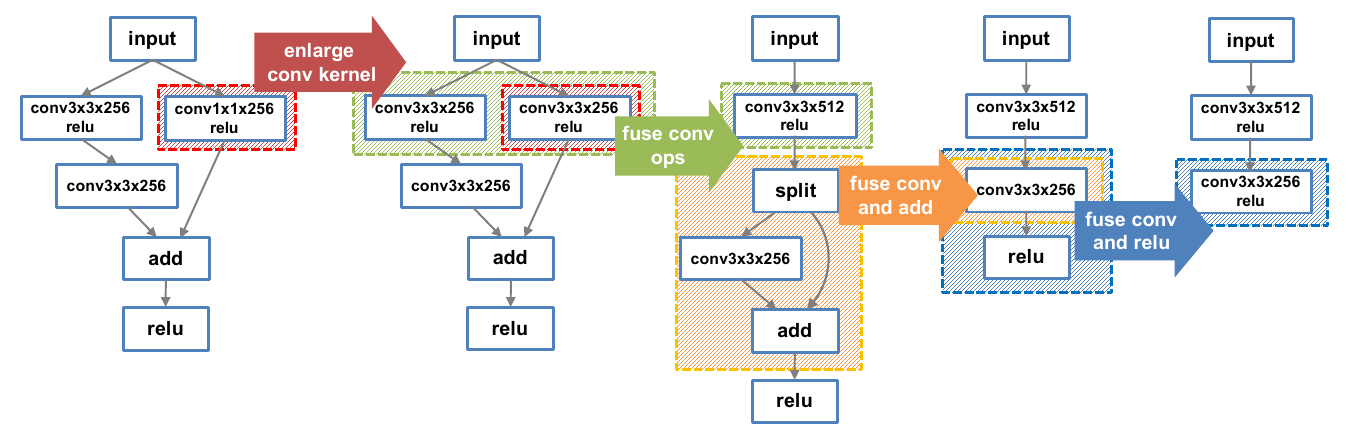
\includegraphics[scale=0.3]{resnetExample}
	%\end{center}	
	%\caption{An example from \cite{jia2019} that demonstrates a relaxed graph substitution}
	%\label{resnet}
%\end{figure}

%%\pagebreak

\chapter{Theoretical Background and Literature Review}
%{\large \noindent \bfseries  The Backtracking Algorithm}\\

\section{Deep Learning Compilers and Motivation}
In this section, we give an overview of the general landscape of deep learning compilers, and motivate the need for the endeavor we choose to embark on. Deep Learning compilers essentially aim to specialize existing, but hitherto general, compilation techniques, so as to perform optimizations specific to deep learning and machine learning workloads. Here by \textit{general}, we mean techniques that can be applied across the board for any language as long as it's first converted to some suitable intermediate representation (assuming the transforms need such a requirement, such as the IC being LLVM IR). Since deep learning computational graphs are usually very uniform and limited in terms of their basic operations, optimizing specifically for them becomes not only reasonably tractable but also beneficent. 

\subsection{Intermediate Representations and The current Optimization Scenario}
According to \cite{li2020deep}, a rather generalized pipeline for compilation frameworks, which are much more amenable to such specializations as deep learning, is emerging in the form of MLIR \cite{lattner2021mlir}. The notion behind such a pipeline can be described in the following way:
\begin{itemize}
	\item Computation graphs are usually defined at a coarse granularity consisting of abstract operations such as convolutions and pooling. While improvements can be made by altering graphs on this level, the abstraction makes doing so quite restricting.
	\item On the other hand, when compiled to intermediate representations such as LLVM IR, the operations not only lose their abstraction, but they plummet to a level no longer reminiscent of the domain they are actually specific too, and so nothing can be done beyond general optimizations whicha are anyways done on general purpose languages like C++ or Java. The idea is that different sized ``chunks'' of this IR represent algorithms or structures that are (i) used exclusively in our domain, such as a convolution algorithm (ii) are at an abstraction level lower than or equal to that of computation graphs. If we could somehow expose these ``chunks'' so that they were explicit operations at a level of abstraction below computation graphs, but above machine code, opportunities exist for much more optimization!
	\item MLIR does exactly this, by allowing users to specify multiple, custom, intermediate representations, called \textit{dialects}, which can be deployed seemlessly into a pipeline where one can iteratively lower from one IR to another, doing any necessary processing on the way.
	\item Having these different IRs, exposes potential for optimizations at different levels.
\end{itemize}

Many deep learning compilers \cite{hloir} \cite{halideir} exploits one of these ``levels'' of interemediate representations to do domain specific optimizations. If done at a lower level, they could be optimized for, say, deep learning hardware like Google's TPUs \cite{jouppi2017datacenter}, and if done at a higher level, they may represent, say, operations such as fusing two convolutions.


\subsection{Motivation for Non-Greedy Approaches}
A lot of research in deep learning compilers has expanded in the following directions:
\begin{itemize}
	\item Creating better IRs for specific applications \cite{li2020deep}.
	\item Optimizing for domain-specific hardware, like TPUs \cite{li2020deep}.
	\item Evolving algorithms that specialize on particular kinds of inputs, for example, Graph Neural Networks \cite{wu2024hector}, which are build specifically to make explicit, graph-like relations in a given problem. 
\end{itemize}

With this literature survey, however, we found that the assumption relating to greedy transformations held true for many cases, and little information was available on non-greedy approaches to optimizing programs. Furthermore, most, if not all, of the aforementioned threads of research already have working implementations on well-reputed libraries such as TensorFlow \cite{tf2016}, PyTorch \cite{pytorchdocs}, and ONNX Runtime \cite{onnxoptimizer} and hence, wouldn't benefit much from another nudge in that same direction. With that in mind, we aim to explore this space of greedy optimizations and replicate results given in \cite{jia2019}.

%{\large \noindent \bfseries  Proposed Methodology}\\
\chapter{Proposed Methodology}

There are essentially three major facets involved in coming up with an implementation for relaxed graph substitutions - implementing the different graph substitution functions that take a graph as an instance and output a modified graph, a backtracking search algorithm that searches the set of all possible semantically correct graph transforms, and the cost function we will use to guide our backtracking search. These can be illustrated with an example as below.

\section{Motivating our Approach Using an Example}
We use an example from a ResNet \cite{he2016} module ( figure \ref{resnet} ) to illustrate our strategy. Each arrow represents a graph substitution that produces a graph \textit{equivalent} to its input, where equivalence is defined as the following: two graphs $\mathcal{G}_1$ and $\mathcal{G}_2$ are said to be equivalent if they produce the same outputs for an arbitrary input. The first substitution pads a 1x1 convolution kernel to form a 3x3 one, potentially reducing the performance by introducing more operations. However, doing so enables further node fusions which, as we can see, results in a computational graph giving better performance than what we started with. 

There is also the need to ensure semantic correctness of these transformations, as each change must retain the original functionality of the model. After applying the transformations, the modified computational graph must give identical outputs for any given input. In a large model, even small numerical errors can accumulate and lead to significant drops in accuracy because there is a possibility that the model's performance gets better but the results that are received are incorrect. \\

\begin{figure}[ht!]
	\begin{center}
		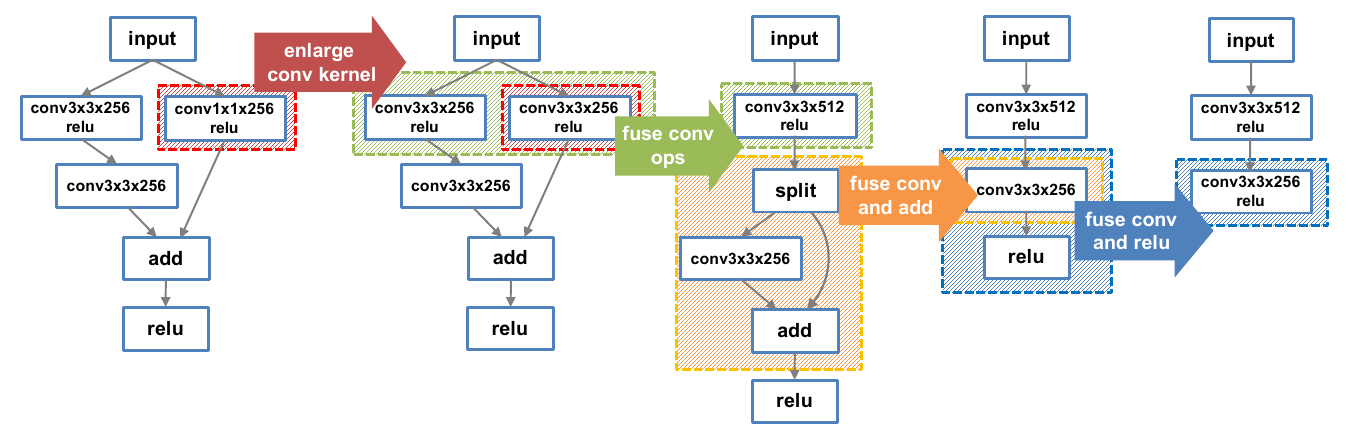
\includegraphics[scale=0.4]{resnetExample}
	\end{center}	
	\caption{An example from \cite{jia2019} that demonstrates a relaxed graph substitution}
	\label{resnet}
\end{figure}

\section{The backtracking Algorithm} \label{backtracking}

		We take the following approach to search through the space of possible graph transformations:
		\begin{enumerate}
			\item Consider a list of possible graph transformations, $T$. At any given point in the algorithm, let $\mathcal{G}$ be the current intermediate graph version. We maintain a priority queue of intermediate graphs, ordered by their \textit{cost}, defined by a heuristic (in our case, this is simply the execution time).
			\item In each iteration:
				\begin{enumerate}
					\item We dequeue to get the next candidate intermediate representation $\mathcal{G}$. 
					\item For each optimization $t_i$ in $T$, we apply $t_i$ on $\mathcal{G}$ to obtain some equivalent graph $\mathcal{G}'$. If $cost(\mathcal{G}') < cost(\mathcal{G})$, we set $\mathcal{G} = \mathcal{G}'$. Else if $cost(\mathcal{G}') < \alpha \cdot cost(\mathcal{G})$, where $\alpha$ is a hyperparameter defined by the user (greater than one), then $\mathcal{G}'$ is considered to be a valid candidate for further search, and is added to the priority queue.
					\item $\alpha$ helps define how much of a performance decrease we can tolerate. This value can't be too high so as to avoid blowing up the search space, and hence, the time it takes for our algorithm to find a beneficial sequence of graph transformations.
				\end{enumerate}

			\item The above is repeated until there are still graphs to process in the queue.

		\end{enumerate}
	\section{Diving Into the Transformations}
		% tensorflow didn't have transforms we could work off of, so went with the paper's example
		% deep dive in the transforms
 Initially, we wanted to look for graph transformations that were already available in any of the deep learning frameworks, such as PyTorch, TensorFlow, etc. But after going deep into the implementations of the transformations provided by the TensorFlow XLA, we noticed that every transformation provided by the deep learning frameworks always improves performance and never degrades it, which dismisses the prospect of relaxed substitutions. Hence, we decided to implement the transformations provided in the \cite{he2016}.
		% tensorflow didn't have transforms we could work off of, so went with the paper's example
		% deep dive in the transforms
		\subsection{Kernel Expansion}

% enlarge conv kernel figure
\begin{figure}[ht]
\centering
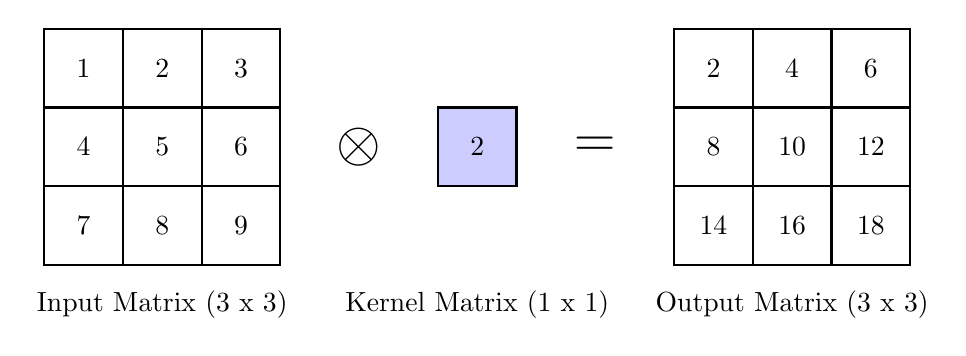
\begin{tikzpicture}
    % Define the block size
    \def\blocksize{1}

    \foreach \i in {0, 1, 2} {
        \foreach \j in {0, 1, 2} {
            \pgfmathtruncatemacro\result{(2-\j)*3+\i+1}
            \draw[thick] (\i*\blocksize, \j*\blocksize) rectangle +(\blocksize, \blocksize);
            \node at (\i*\blocksize + 0.5*\blocksize, \j*\blocksize + 0.5*\blocksize) {\result};
        }
    }

    \node at (4.0, 1.5) {\huge $\otimes$};

    \draw[thick, fill=blue!20] (5.0, 1.0) rectangle +(\blocksize, \blocksize);
    \node at (5.0 + 0.5*\blocksize, 1.0 + 0.5*\blocksize) {2};

    \node at (7.0, 1.5) {\huge =};

    \foreach \i in {0, 1, 2} {
        \foreach \j in {0, 1, 2} {
            \pgfmathtruncatemacro\result{((2-\j)*3+\i+1)*2}
            \draw[thick] (8.0 + \i*\blocksize, \j*\blocksize) rectangle +(\blocksize, \blocksize);
            \node at (8.0 + \i*\blocksize + 0.5*\blocksize, \j*\blocksize + 0.5*\blocksize) {\result};
        }
    }

    % Labels
    \node at (1.5, -0.5) {Input Matrix (3 x 3)};
    \node at (5.5, -0.5) {Kernel Matrix (1 x 1)};
    \node at (9.5, -0.5) {Output Matrix (3 x 3)};

\end{tikzpicture}

\label{kernelExpansion0}
\caption{Convolution Operation with a 1x1 kernel matrix, a padding of zero, and stride 1}
\end{figure}

\begin{figure}[ht]
\centering
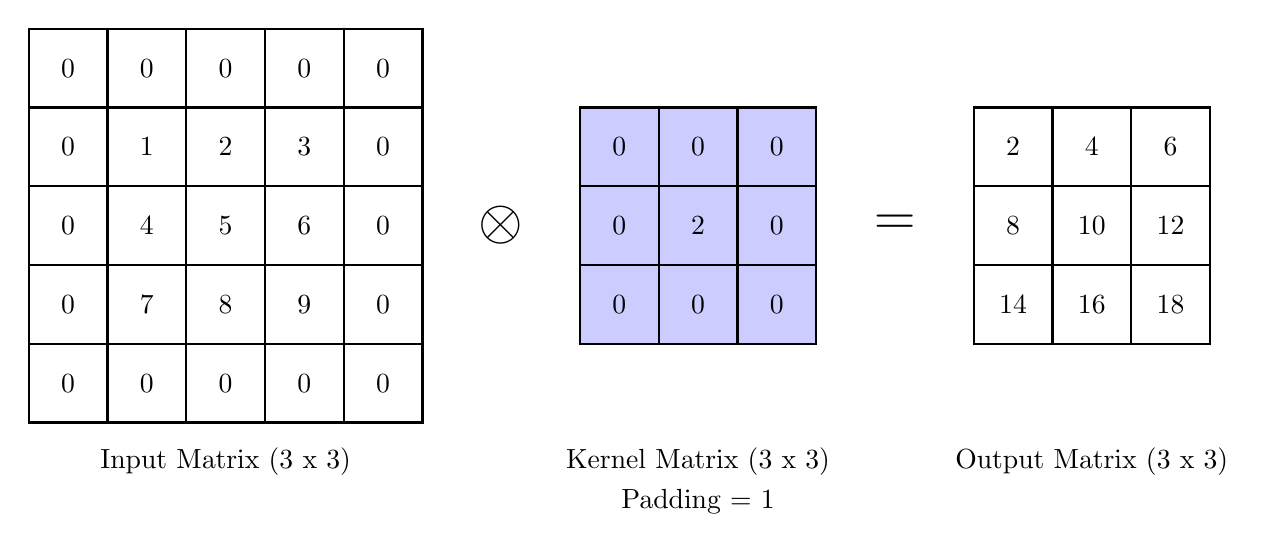
\begin{tikzpicture}
    % Define the block size
    \def\blocksize{1}

    \foreach \i in {0, 1, 2, 3, 4} {
        \foreach \j in {0, 1, 2, 3, 4} {
            \pgfmathtruncatemacro\result{(3-\j)*3+\i}
            \pgfmathtruncatemacro\finalresult{ifthenelse(\i==0 || \j==0 || \i==4 || \j==4, 0, \result)} % Apply conditions
            \draw[thick] (\i*\blocksize, \j*\blocksize) rectangle +(\blocksize, \blocksize);
            \node at (\i*\blocksize + 0.5*\blocksize, \j*\blocksize + 0.5*\blocksize) {\finalresult};
        }
    }

    \node at (6.0, 2.5) {\huge $\otimes$};

    \foreach \i in {0, 1, 2} {
        \foreach \j in {0, 1, 2} {
            \pgfmathtruncatemacro\result{0}
            \pgfmathtruncatemacro\finalresult{ifthenelse(\i==1 && \j==1, 2, \result)} % Apply conditions
            \draw[thick, fill=blue!20] (7 + \i*\blocksize, 1 + \j*\blocksize) rectangle +(\blocksize, \blocksize);
            \node at (7 + \i*\blocksize + 0.5*\blocksize, 1 + \j*\blocksize + 0.5*\blocksize) {\finalresult};
        }
    }

    \node at (11.0, 2.5) {\huge =};

    \foreach \i in {0, 1, 2} {
        \foreach \j in {0, 1, 2} {
            \pgfmathtruncatemacro\result{((2-\j)*3+\i+1)*2}
            \draw[thick] (12.0 + \i*\blocksize, 1.0 + \j*\blocksize) rectangle +(\blocksize, \blocksize);
            \node at (12.0 + \i*\blocksize + 0.5*\blocksize, 1.0 + \j*\blocksize + 0.5*\blocksize) {\result};
        }
    }

    % Labels
    \node at (2.5, -0.5) {Input Matrix (3 x 3)};
    \node at (8.5, -0.5) {Kernel Matrix (3 x 3)};
    \node at (8.5, -1.0) {Padding = 1};
    \node at (13.5, -0.5) {Output Matrix (3 x 3)};

\end{tikzpicture}

\label{kernelExpansion1}
\caption{A convolution operation after padding both, the kernel and the image.}
\end{figure}

               The substitution \verb|enlarge_conv_kernel| increases the kernel size from 1x1 to a larger 3x3 size. This change enables further transformations that can lead to improved performance. However, as previously mentioned, simply increasing the kernel size does not guarantee correctness. \\

              Let us assume the initial kernel size is $f$, and the final kernel size is $f+k$, where we are increasing the kernel size by $k$. The initial padding is $p$, and the final padding is $p'$. The input size is $n$.

               \begin{equation}
                    \frac{n+2p-f}{s} + 1 = \frac{n+2p^\prime-(f+k)}{s} + 1
                \label{eq:enlarge1}
                \end{equation}

                \begin{equation}
                    2p-f= 2p^\prime-(f+k)
                \label{eq:enlarge2}
                \end{equation}

                \begin{equation}
                    \boxed{p^\prime = p + \frac{k}{2}}
                \label{eq:enlarge2}
                \end{equation}

                Hence, enlarging the kernel will also require adding padding to the input in the convolution operation to maintain the same output dimensions.

            \subsection{Convolution Fusions}
            Convolution Fusions combine multiple convolution oeprations into a single, more efficient oepration. This approach aims to reduce the number of operations and memory access overhead by merging sequential convolutional layers.

    \begin{figure}[ht]
    \centering
    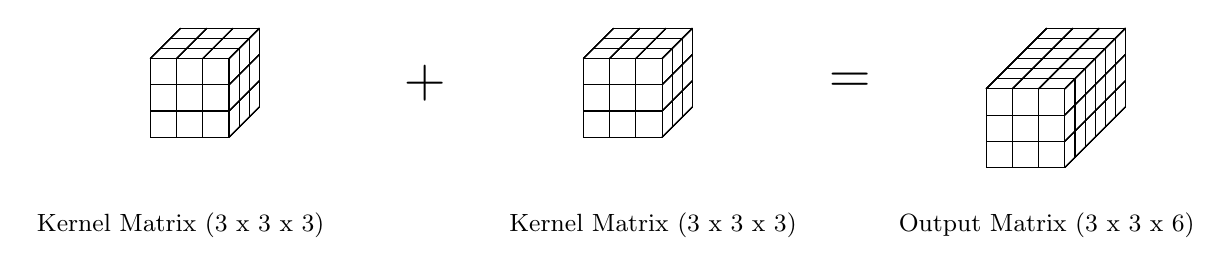
\begin{tikzpicture}
        % First Cube
        \foreach \x in {0, 1, 2, 3} {
            \foreach \y in {0, 1, 2, 3} {
                \draw (2.5 + 0, \y/3, 3/3) -- (2.5 + 3/3, \y/3, 3/3); % Horizontal lines
                \draw (2.5 + \y/3, 0, 3/3) -- (2.5 + \y/3, 3/3, 3/3); % Vertical lines on YZ plane
                \draw (2.5 + 3/3, \y/3, 3/3) -- (2.5 + 3/3, \y/3, 0); % Vertical lines on XZ plane
                \draw (2.5 + \y/3, 3/3, 3/3) -- (2.5 + \y/3, 3/3, 0); % Horizontal lines on XY plane
                \draw (2.5 + 3/3, 0, \y/3) -- (2.5 + 3/3, 3/3, \y/3); % Vertical lines on XZ plane
                \draw (2.5 + 0, 3/3, \y/3) -- (2.5 + 3/3, 3/3, \y/3); % Horizontal lines on XY plane
            }
        }

        \node at (5.6, 0.3) {\huge +};

        % Second Cube
        \foreach \x in {0, 1, 2, 3} {
            \foreach \y in {0, 1, 2, 3} {
                \draw (8.0, \y/3, 3/3) -- (8.0 + 3/3, \y/3, 3/3); % Horizontal lines
                \draw (8.0 + \y/3, 0, 3/3) -- (8.0 + \y/3, 3/3, 3/3); % Vertical lines on YZ plane
                \draw (8.0 + 3/3, \y/3, 3/3) -- (8.0 + 3/3, \y/3, 0); % Vertical lines on XZ plane
                \draw (8.0 + \y/3, 3/3, 3/3) -- (8.0 + \y/3, 3/3, 0); % Horizontal lines on XY plane
                \draw (8.0 + 3/3, 0, \y/3) -- (8.0 + 3/3, 3/3, \y/3); % Vertical lines on XZ plane
                \draw (8.0, 3/3, \y/3) -- (8.0 + 3/3, 3/3, \y/3); % Horizontal lines on XY plane
            }
        }

        \node at (11, 0.3) {\huge =};

        % Cuboid (with correction)
        \foreach \x in {0, 1, 2, 3} {
            \foreach \y in {0, 1, 2, 3} {
                % Draw the front face
                \draw (13.5, \y/3, 2) -- (13.5 + 1, \y/3, 2); % Top horizontal on front face
                \draw (13.5 + \y/3, 0, 2) -- (13.5 + \y/3, 1, 2); % Side vertical on front face
                \draw (13.5 + 1, \y/3, 2) -- (13.5 + 1, \y/3, 0); % Right vertical on front face
                \draw (13.5 + \y/3, 1, 2) -- (13.5 + \y/3, 1, 0); % Bottom horizontal on front face

            }
        }

        % Add height edges for the depth of the cuboid
                \draw (13.5 + 1, 0, 2/6) -- (13.5 + 1, 0+1, 2/6); % Right front vertical edge
                \draw (13.5 + 1, 0, 4/6) -- (13.5 + 1, 0+1, 4/6); % Right front vertical edge
                \draw (13.5 + 1, 0, 6/6) -- (13.5 + 1, 0+1, 6/6); % Right front vertical edge
                \draw (13.5 + 1, 0, 8/6) -- (13.5 + 1, 0+1, 8/6); % Right front vertical edge
                \draw (13.5 + 1, 0, 10/6) -- (13.5 + 1, 0+1, 10/6); % Right front vertical edge
                \draw (13.5 + 1, 0, 0) -- (13.5 + 1, 0+1, 0); % Right front vertical edge

                \draw (13.5, 1, 1) -- (13.5+1, 1, 1); % Top horizontal on front face
                \draw (13.5, 1, 2/6) -- (13.5+1, 1, 2/6); % Top horizontal on front face
                \draw (13.5, 1, 4/6) -- (13.5+1, 1, 4/6); % Top horizontal on front face
                \draw (13.5, 1, 8/6) -- (13.5+1, 1, 8/6); % Top horizontal on front face
                \draw (13.5, 1, 10/6) -- (13.5+1, 1, 10/6); % Top horizontal on front face
                \draw (13.5, 1, 0) -- (13.5+1, 1, 0); % Top horizontal on front face

    \node at (2.5, -1.5) {\small Kernel Matrix (3 x 3 x 3)};
    \node at (8.5, -1.5) {\small Kernel Matrix (3 x 3 x 3)};
    \node at (13.5, -1.5) {\small Output Matrix (3 x 3 x 6)};

    \end{tikzpicture}

	\label{convFusion0}
	\caption{Fusing two kernel matrices}
\end{figure}

            The fusing of convolution layers can only be done if the following conditions are satisfied:

            \begin{tcolorbox}[colback=gray!5!white, colframe=gray!75!black, title=Constraints on the Source Graph]
            \begin{itemize}[left=0pt]
                \item \verb|conv1.kernel == conv2.kernel|
                \item \verb|conv1.stride == conv2.stride|
                \item \verb|conv1.padding == conv2.padding|
            \end{itemize}
        \end{tcolorbox}
        
        \begin{tcolorbox}[colback=gray!5!white, colframe=gray!75!black, title=Construct the Target Graph]
            \begin{itemize}[left=0pt]
                \item \verb|conv3.outChannels = conv1.outChannels + conv2.outChannels|
                \item \verb|conv3.weights = concat(conv1.weights, conv2.weights)|
                \item \verb|split.sizes = [conv1.outChannels, conv2.outChannels]|
            \end{itemize}
        \end{tcolorbox}

\subsection{Fusing Conv and Add Nodes}
	  One of the more non-obvious and harder to unpack transformations proved to be the fusion of a Convolutional node and an Add node. The process is best understood by first revisiting concepts of Convolution networks.
	  \begin{figure}[b!]
		\begin{center}
			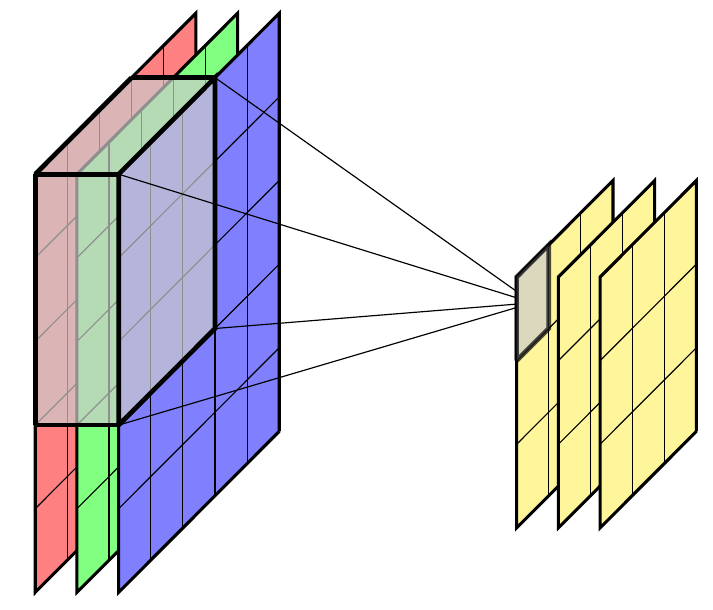
\includegraphics[scale=0.3]{reportImages/CNN_revision_bishop.png}
		\end{center}	
		\caption{An illustration from \cite{bishop2023deep} that shows a  multi-dimensional convolutional filter layer extended to include multiple independent filter channels.}
		\label{cnn_revision}
	\end{figure}
	  \begin{itemize}
		\item An image with $J \times K$ pixels and C channels will be described by a tensor of dimensionality $J \times K \times C$. We introduce a filter described by a tensor of dimensionality $M \times M \times C$ comprising a separate $M \times M$ filter for each of the C channels.
		\item Secondly, we introduce multiple such filters, each detecting a seperate abstract feature in the input image. The number of these specific filters are referred to as the channels of the kernel and are denoted by the third number in the notation $3 \times 3 \times 512$ for a convolutional layer.
		\item For each filter, after performing the convolution operation across all channels of the input image, the resulting C channels are summed to produce the final feature map representing the abstract feature the filter is designed to detect.
	\end{itemize}

	Now with the basis of the convolutional approach laid down, we can explore the optimization. The input is a $3 \times 3 \times 512$ image which was formed after fusing two $3 \times 3 \times 256$ convolutional operations together. The first 256 channels out of the 512 denote the input that came from Conv1 and the rest 256 denote the channels that came from Conv2. As figure \ref{resnet} shows, the expected behaviour is for the Conv1 channels to undergo one more convolution, say Conv4, and then simply get added to the Conv2 output.

	The optimization here is to cleverly modify the kernel matrix of a new Conv operation, call it Conv3, that includes within it the Convolution operation on Conv1 channels and subsequent addition. The approach is as follows:
	  \begin{itemize}
		\item In Conv3, there are 256 different filters. Each of these filters is responsible for extracting some abstract feature.
		\item Each of these filters has 512 channels, 256 devoted to processing the channels consolidated from Conv1 and the remaining 256 for processing the add.
		\item Note that each filter within the Conv4 layer has 256 channels within it to handle the 256 input channels from Conv1.
		\item The fusion is accomplished in two steps. The first is to have the first 256 channels of Conv3 be initialized with the weights of the corresponding channel in the $3 \times 3 \times 256$ Conv4.
		\item Now, we know that, per abstract feature, after carrying convolution over all channels, the final feature map is a result of summing up over all the channels. In our current arrangement the first 256 channels, when summed up, will give the output feature map corresponding to performing Conv4 for that abstract feature. The remaining part is to add to this sum precisely the channel that corresponds to Conv2, that, when added, will simulate doing a sum post convolution.
		\item The trick here is to use the \textbf{identity kernel}, which simply outputs the input as is without modification. It is also called a do-nothing kernel.
		\[ I = 
	\begin{bmatrix}
	0 & 0 & 0 \\
	0 & 1 & 0 \\
	0 & 0 & 0
	\end{bmatrix}
	\]
		\item Let us make a few constructs:
		\begin{itemize}
			\item Let 0 represent a 3x3 kernel filled with all zeros.
			\item Let each row of the matrix represent the kernel corresponding to one of the 256 abstract features in Conv3.
			\item Let $f_{i,j}$ denote a $k \times k$ filter for abstract feature $i$ and channel $j$.
		\end{itemize} . 
		\[
			\begin{bmatrix}
					f_{1,1} & f_{1,2} & f_{1,3} & \cdots & f_{1,256} & I & 0 & 0 & \cdots & 0\\
					f_{2,1} & f_{2,2} & f_{2,3} & \cdots & f_{2,256} & 0 & I & 0 & \cdots & 0\\
					\vdots & \vdots & \vdots & \vdots & \vdots & \vdots & \vdots & \vdots & \cdots & \vdots \\
					f_{256,1} & f_{256,2} & f_{256,3} & \cdots & f_{256,256} & 0 & 0 & 0 & \cdots & I
			\end{bmatrix}
	\]
	\item The above kernel matrix can be seen as the original Conv4 weight matrix concatenated with an "Identity" matrix. This identity matrix is actually a matrix of matrices where the diagonal elements are identity kernels.
	\end{itemize}
	By configuring the last 256 channels to either the identity matrix  $I$ or zero, as shown in the matrix above, we can selectively sum the layers that would have been added in the original computational graph.

	\section{The Cost Model}
		
		% Explain the need for evaluating it statically
		% FLOPS
		% Execution time
		
	When comparing the expected performance of intermediate graphs, $\mathcal{G'}$, we cannot simply run the inference on them and compare execution times because an exhaustive search will go through a vast number of potential graphs. Running them will not only result in an enormous amount of computation overhead, but also might involve convoluted problems related to memory latencies and slow I/O operations, making such a strategy quite impracticable. Furthermore, it might be better to have an algorithm that is more amenable to a flexible cost function, that optimizes for not necessarily execution time, but also other metrics such as FLOP or Memory accesses. As a result, a flexible, static cost estimation strategy must be developed. The following are some considerations to keep in mind:
	\begin{enumerate}
		\item \textbf{FLOP:} In order to measure the number of Floating Point Operations for some algorithm, it's essential to analyze its low-level implementation intricately, including costs incurred by library functions and user-defined functions alike. Since for our implementation, we plan to use APIs provided by tools like ONNX and TensorFlow to support our model, doing such an analysis is quite infeasible, and hence, estimating FLOP is left as a potential future work.
		\item \textbf{Execution Time:} Interestingly enough, because deep learning computational graphs are quite uniform in structure, it is possible to give decent statically-determined approximations of the execution time, if we have with us, pre-determined (through experiments) execution times for primitive operations given certain parameters. For example, the runtime for a convolution operation on kernel size K, with padding P and stride S will stay relatively the same for another convolution in the graph having the same kernel size, padding and stride. How these primitive execution times are composited, however, is something we plan to do as a part of this project, and has not been well thought at the moment.
		\item \textbf{Other metrics:} Metrics such as memory usage may also be optimized, and may even pose a tradeoff with some other metrics. Estimating these has been left as potential future work.
	\end{enumerate}

\chapter{Future Work}
The preceeding section explicated our understanding of what implementing an exhaustive-search non-greedy optimization will entail. Hence, we now plan to concretely implement each of these three facets as follows:

	\section{Implementing Transformations for ONNX}
	To create custom examples using the ONNX (Open Neural Network Exchange) graph, we leverage the ONNX helper API provided by \cite{onnxpython}. This powerful API enables us to generate custom tensors through the \verb|make_tensor| function and to define new nodes within the computation graph using the \verb|make_node| function from \verb|onnx.helper|. 

	Furthermore, to apply transformations to the ONNX graph, the attributes and methods available in \verb|onnx.onnx_ml_pb2.ModelProto| part of Python's ONNX library—prove to be exceptionally effective.

	Our current efforts at implementation can be seen on this public GitHub repository.

	\section{Regarding the Backtracking Algorithm}
	The backtracking algorithm mentioned in \ref{backtracking} is the essential part of our implementation. It decides which graph transformations are good depending on the \verb|cost_model| and the \verb|alpha| parameter. The algorithm uses a \verb|transform| method, which takes in the ONNX graph representation and applies it to the node. The modification of the graph is done by using a graph traversal algorithm quite similar to Depth First Search. During the search, we also use a \verb|verifier|, which checks whether the given node can be applied a given transformation, hence generating new transformed graphs that are pushed into the queue.

	\section{Cost Model}
	This is a critical section where we need to find a way to take, say, costs of primitive nodes given certain parameters, and merge them so as to accurately predict the execution time (say) of the entire subgraph. This might include considerations such as memory latencies, or it might be intractable, in which case the only solution would be to take also the representations of those ``merged'' operations, and pre-compute their runtime estimates like other priimitive operations. This feasibility check is yet to be made.

\chapter{Conclusion}
In this report, we explained the notion of non-greedy optimizations, motivated their need, and gave an exposition on our attempt at implementing the same, with our work being based on \cite{jia2019}. We saw using an example, how allowing interemediate results that are less optimal, we can find paths that ultimately lead to graphs better than what we would have obtained using a greedy approach. Because individual heuristics for such special cases would lead to a convoluted software, a backtracking algorithm is used to exhaustively search the entire space of graphs enabled by a predetermined set of transformations. At a given iteration, the backtracking algorithm estimates the performance of an intermediate result using a \textit{cost model}, and uses a parameter $\alpha$ to set how relaxed of a substitution we can tolerate, based on factors such as external time-bounds or performance bounds. Finally, we presented our plan regarding the next step in this endeavor, that is to implement certain transformations, the backtracking algorithm and the cost model on an existing platform such as ONNX.

%\begin{enumerate}

	%\item The first step would be to finalize a set of graph transformations we will be working with (i.e. the set $T$ in the earlier algorithm). We initially construted the initial computation graph shown in figure \ref{resnet} using the ONNX Python API \cite{onnxpython}, and explored the graph transformations made available by the ONNX Optimizer \cite{onnxoptimizer} through a simple backtracking algorithm. That being said, since ONNX provides \textit{optimizations} and not \textit{transformations}, each available transform is bound to improve performance for most if not all input graphs. This renders the purpose of our algorithm moot. This is why, we now plan to explore the transformations made available through the TensorFlow \cite{tf2016} API which also provides a tool to write custom transforms.
	%\item Once a set of Tensorflow transforms are shortlisted, we can move on to analyze the feasibility of, and then potentially implement, the two latter transforms mentioned in figure \ref{resnet}, which currently don't have implementations in TensorFlow. 
	%\item We then create a test suite consisting of small computation graphs that demonstrate the abilities of our algorithm.
	%\item Once the aforementioned stages are successful, we will then benchmark our backtracking implementation against the aforementioned test suite, and analyze the results.
	%\item Based on the results obtained, we then aim to tweak the cost model that approximates the cost function for an input graph so as to consider other parameters such as FLOPS or memory consumed.
	%\item The above steps will hopefully yield a model that is successful with regard to small input computation graphs. In order to scale this system to work for existing models, which have massive computation graphs that are bound to blow up the search space exponentially, we plan to create a \textit{graph splitting} algorithm that divides the computation graph into smaller sub-graphs. Each sub-graph can then be optimized through the earlier algorithm. In \cite{jia2019}, the metric used to find partitioning-boundaries is a parameter called $Cap(N)$, which, for a given node $N$, tells us the number of graph transformations thwarted if the graph were split through this node. Since we want the least number of thwarted transforms, the paper then uses the max-flow algorithm \cite{cormen2009introduction} to find partitioning boundaries.
	%\item The paper also mentioned that this min-cut algorithm is not necessarily optimal for all models. Hence, there is scope of improvement with regard to defining better graph-splitting heuristics. We see this as possible future work.

%\end{enumerate}

%\addcontentsline{toc}{chapter}{References}
\bibliographystyle{plain}
\bibliography{refs}

%\begin{center}
%\begin{tabular}{@{}p{.5in}p{4in}@{}}
%& \hfill \\
%& \hfill \\
%& \hrulefill \\
%& Shri. R. P. Gohil \\
%& Associate Professor, DoCSE, SVNIT\\
%\end{tabular}
%\end{center}

\chapter*{Acknowledgements}
\addcontentsline{toc}{chapter}{Acknowledgements}

Any palpable progress with this work wouldn't have been possible without Prof. R. P. Gohil's guidance on a very fundamental level: we needed to base our goals on a concrete feasibility analysis rather than quixotic assumptions of glory. We really did face quite a few contingencies even after narrowing our focus down to something realistic, but, thanks to his prudent reminder, we are now on a better trajectory going forward. 

\end{document}
